\chapter{Architektur}

	Beim hier verwendeten Entscheidungstemplate handelt es sich um das "`IBM UMF Template for Decision Log"' \cite{hand_ibm_2008}.
	
	\section{Erweiterung CDAR}
		Für das Anbinden ans \cdar\ gibt es verschiedene Möglichkeiten.
		Wir haben uns für eine eigene Serverkomponente, ein eigenes Userinterface und eine eigene Persistenz entschieden.
		Die Alternativen und die Details zu diesem Entscheid sind nachfolgend aufgeführt.
		
		\decision{
			\decisionHeader{1}{Erweiterung \cdar\ / Integration}{Integration}{Architektur design}
		}{
			\decisionContent{Eigene Serverkomponente, keine UI Integration, eigene Persistenz}
			{In welcher Art soll \eeppi\ mit dem \cdar\ integriert werden?}
			{Die \cdar\ Authentisierungs-API erlaubt das Bauen eines SSO über mehrere Applikationen hinweg.}
			{Diese Entscheidung beeinflusst die Möglichkeiten der Technologiewahl, der zu nutzenden Schnittstellen und Komponenten und ist daher Grundlegend für weitere Entscheidungen.}
			{
				Jede der Entscheidungen (Serverkomponente, Clientapplikation, Persistenz) kann unabhängig der andern zwei getroffen werden in diesem Fall. Darum sind hier nur die Alternativen der jeweiligen einzelnen Entscheidungen und nicht alle Kombinationen aufgelistet:
				\begin{description}					
					\item[\cdar\ UI erweitern]
					Integration der \eeppi-Funktionalität ins UI des \cdar.			
					\begin{description}
						\item[Vorteile] Nur eine Applikation für Benutzer
						\item[Nachteile] \cdar\ UI muss angepasst werden, \eeppi\ ist vom \cdar\ abhängig
					\end{description}
					
					\item[Serverkomponente ersetzen]
					\eeppi\ bildet eine gemeinsame neue Serverkomponente, die diejenige des \cdar\ ersetzt.
					\begin{description}
						\item[Vorteile] Einheitlichen Unterbau für \cdar\ und \eeppi, nur eine Schnittstelle, nur eine Serverkomponente, einfachere Installation
						\item[Nachteile] Sehr aufwändig, da die \cdar\ Server Komponente viel zu ersetzende Logik beinhaltet, \eeppi\ ist mit \cdar\ gekoppelt.
					\end{description}
					
					\item[\cdar\ Persistenz erweitern]
					\eeppi\ nutzt die Persistenz des \cdar\ und erweitert diese.
					\begin{description}
						\item[Vorteile] Einfachere Wartung, nur eine Persistenz für Backup
						\item[Nachteile] Kopplung von \eeppi\ an \cdar
					\end{description}
				\end{description}
			}
			{
				\eeppi\ soll die \cdar-API und den Login-Mechanismus benutzen. \eeppi\ besitzt allerdings eine eigene Server- sowie UI-Komponente und eine eigene Persistenz. 
				\begin{description}
					\item[Vorteile] \
						\begin{itemize}
							\item Die Persistenz kann im gleichen System wie \cdar\ untergebracht sein, kann aber auch auf einem komplett andern Host laufen.
							\item Es sind keine Anpassungen an \cdar\ notwendig, weder an der Persistenz, der Serverkomponente noch am UI.
							\item \eeppi\ ist Unabhängig vom \cdar\ und könnte auch mit einer andern Applikation als das \cdar\ gekoppelt werden.
							\item Trotz der Unabhängigkeit ist SSO für Benutzer möglich.
						\end{itemize}
					\item[Nachteile] Benutzer müssen zwei Applikationen nutzen (andere URL als \cdar), die Installation ist komplizierter
				\end{description}
				Im Laufe der Prototypenphase wurde dem Team mitgeteilt, 
				das das \cdar\ durch eine schlanke Schnittstellenapplikation ersetzt wird, 
				die ihre Daten von der Enterprise Architect Erweiterung "`ADMentor"' bezieht. 
				Diese Veränderung bestätigte die Entscheidung für die gewählte Variante, 
				bedingte allerdings, das \eeppi\ selbst eine Benutzerverwaltung besitzen muss.
			}
			{}
			{Die Schnittstelle für den Authentisierungsservice und die Datenquelle (Anbindung \cdar) muss generisch und konfigurierbar gestaltet sein.}
			{"`Server Technologie"', "`Tier Architektur"'}
		}
		

	\section{Architekturübersicht}
	
	
	\section{Tier-Architektur}
		Aufgrund der Einschränkung von Technologie und den existierenden Komponenten des \cdar's stehen drei mögliche Tier-Architekturen zur Auswahl.
		Die hier verwendeten Begriffe stützen sich auf von Prof. Dr. Zimmermann verwendete Begriffe in der HSR Vorlesung "`Application Architecture"'\cite{prof._dr._zimmerman_layers_2014}.		
		
		\begin{figure}[H]
			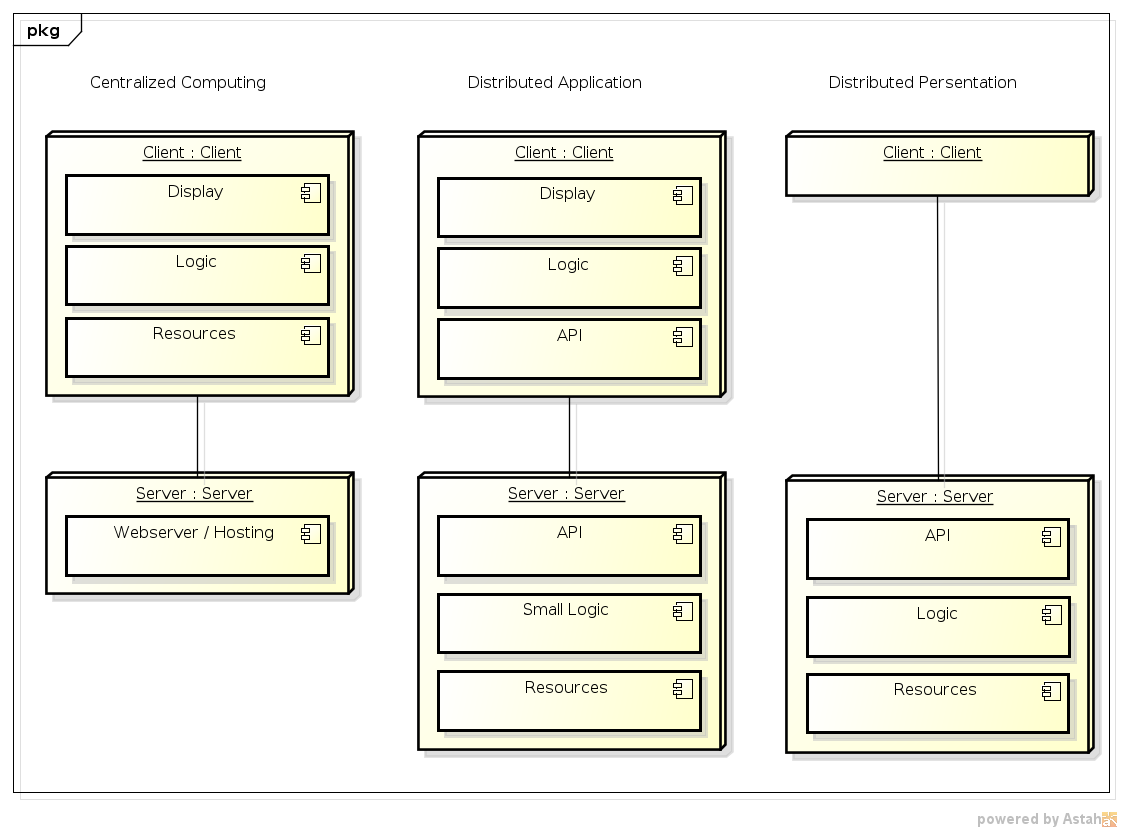
\includegraphics[width=\textwidth]{architecture/media/img/tierArchitecture.png}
			\centering
			\caption{Architektur Varianten}
			\label{fig:tierArchitecture}
		\end{figure}
		\begin{description}
			\item[1-Tier Structure: Centralized Computing (Client-only Application)]
				Die Serverkomponente übernimmt lediglich das Ausliefern einer WebApp. 
				Die WebApp bezieht die Daten direkt aus externen Schnittstellen. 
				Persistenz findet dezentral auf dem Client statt in Form von File Persistence oder 
				Persistence durch das Framework (z.B. HTML5 Storage).
				
			\item[2-Tier Structure: Distributed Application (Single Page App)]
				Die Serverkomponente übernimmt Persistenz sowie minimale Logik (z.B. Login).
				Presentation und Logik werden von der Client Komponente übernommen.
				
			\item[2-Tier Structure: Distributed Presentation]
				Persistenz, Logik und Presentation werden vom Server übernommen.
				Die Presentation wird fertig aufbereitet an den Client gesendet (z.B. HTML Page).
				Es gibt keine aktiven Komponenten auf dem Client ausser asyncron nachladenden Skripten.
				
		\end{description}
	
		\decision{
			\decisionHeader{1}{Tier Architektur}{Architektur}{Architektur design}
		}{
			\decisionContent{Distributed Application (Single Page Application)}
			{Welche Tier Architektur soll für \eeppi\ gewählt werden?}
			{}
			{Diese Entscheidung ist wichtig, damit eine möglichst lose Kopplung \& hohe Flexibilität auch für zukünftige, auf \eeppi\ und \cdar\ aufbauende Applikationen, erreicht wird und der Grundstein für Technologieentscheidungen gelegt wird.}
			{"`Centralized Computing"', "`Distributed Presentation"'}
			{"`Distributed Application"' ermöglicht, die bestehende Serverlogik des \cdar\ zu nutzen, 
				eine Serverseitige (zentralisierte) Persistenz anzubieten sowie dem Benutzer eine schnelle und unabhängige Applikation zur Verfügung zu stellen, 
				die die Rechenleistung des Clients beansprucht, sodass der Server und dessen Kosten schlank gehalten werden können.
				Da die App vom Server ausgeliefert wird, kann sie zentral von dort aus verwaltet, gewartet und kontrolliert werden.}
			{}
			{}
			{}
		}
		
	\section{Session State}
		Eine Session (Session State Pattern\footnote{\url{http://www.bettersoftwaredesign.org/Design-Patterns/Enterprise-Application-Architecture-Patterns/Session-State-Patterns}}) kann auf dem Client abgelegt werden, auf dem Server oder persistiert werden.
		
		\decision{
			\decisionHeader{2}{Session State}{Architektur}{Architektur design}
		}{
			\decisionContent{Client Session State}
			{Auf welchem Tier sollen User Sessions gespeichert werden?}
			{}
			{Diese Entscheidung beeinflusst Client wie Server und bestimmt, ob der der Server zustandsbehaftet oder nicht ausgelegt wird.}
			{"`Server Session State"', "`Database Session State"'}
			{"`Client Session State"' ermöglicht es, 
				den Server zustandslos zu implementieren. 
				Dadurch wird eine reine Resourcen-basierte Serverschnittstelle möglich.			
			}
			{}
			{Der Client muss eine Möglichkeit bieten, eine Session zu speichern. Bevorzugt soll dafür ein Session Cookie zum Einsatz kommen.}
			{}
		}